\documentclass{article}

\usepackage{graphicx}
\usepackage{caption}
\usepackage{subcaption}
\usepackage{float}

\begin{document}


%  Indsæt et billede
\begin{figure}[H] 
\begin{center}
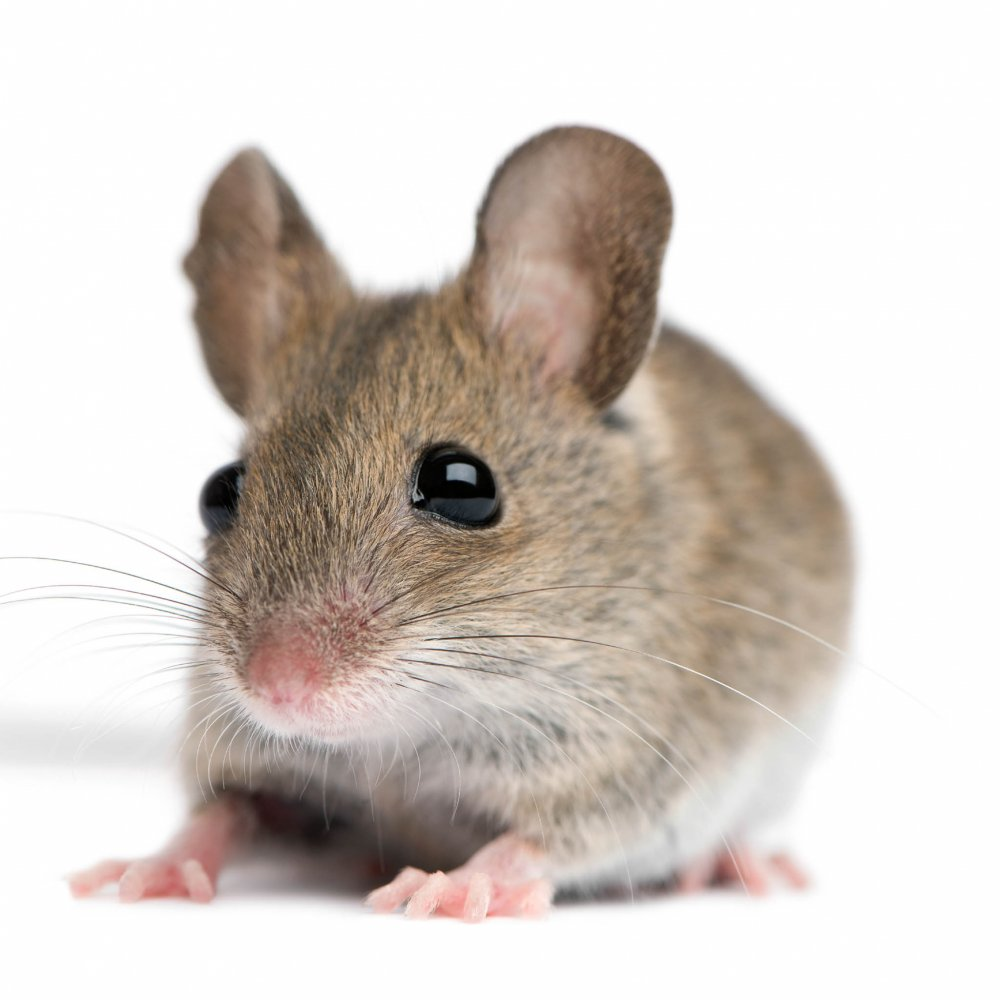
\includegraphics[width=0.7\textwidth]{figures/mus} %indsæt filnavn på mus's plads
\end{center}
\caption{Billedtekst. \cite{mus}} %indsæt kilde på mus's plads
\label{fig:mus} %indsæt label på mus's plads
\end{figure}

%  Indsæt to billeder


\begin{figure}[H]
  \begin{subfigure}[b]{0.5\textwidth}
    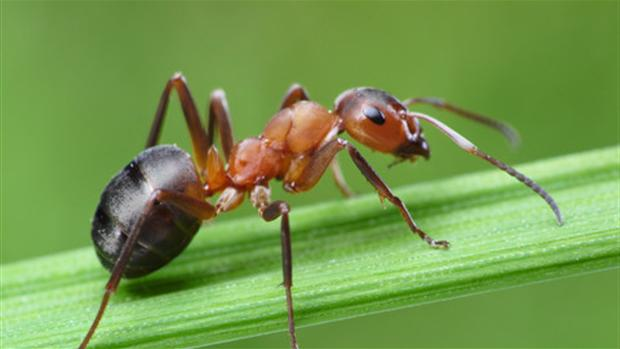
\includegraphics[width=\textwidth]{figures/myre} %indsæt filnavn på myre's plads
    \caption{Billedtekst. \cite{myre}} %indsæt kilde på myre's plads
    \label{fig:myre} %indsæt label på myre's plads
  \end{subfigure}
  \hfill
  \begin{subfigure}[b]{0.5\textwidth}
    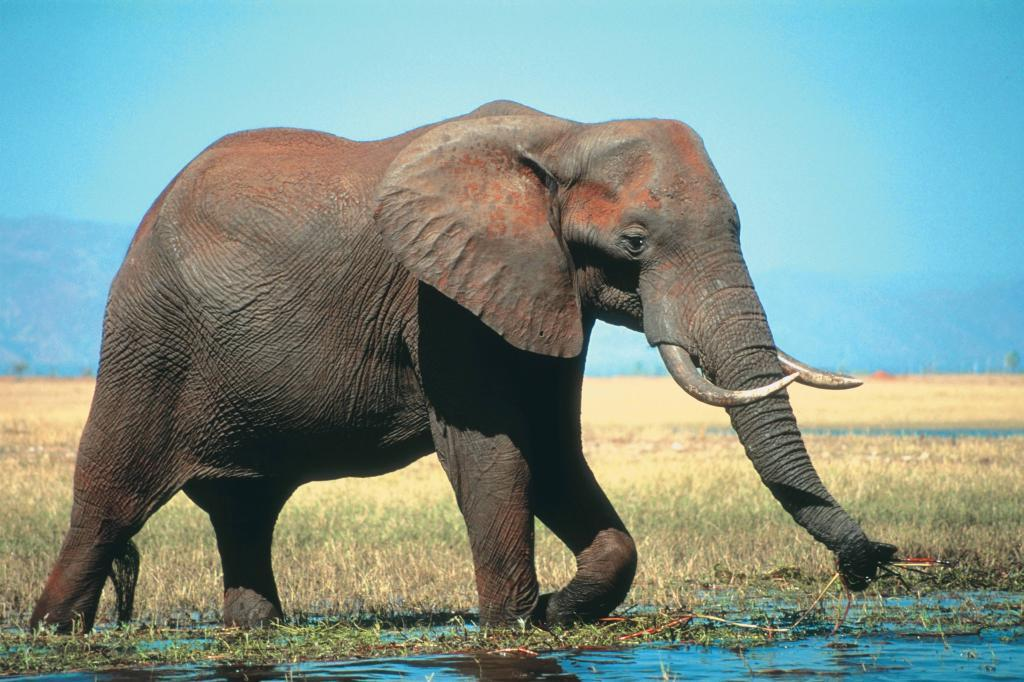
\includegraphics[width=\textwidth]{figures/elefant} %indsæt filnavn på elefant's plads
    \caption{Billedtekst. \cite{elefant}} %indsæt kilde på elefant's plads
    \label{fig:elefant} %indsæt label på elefant's plads
  \end{subfigure}
  \caption{Overordnet billede tekst\cite{myre_elefant}} %indsæt kilde på myre_elefant's plads}
\end{figure}


\end{document}
